\part{Gnu/Linux基础知识篇}
\label{part1}

\chapter{关于本书}
\label{part1:chap1}

GNU/Linux是GNU\index{GNU}计划的支持者与开发者,特别是其创立者Richard
Stallman\footnote{理查德·马修·斯托曼,美国自由软件运动的精神领袖、GNU计
  划以及自由软件基金会的创立者。作为一个著名的黑客,他的主要成就包
  括Emacs及后来的GNU Emacs\index{Emacs},GNU C编译器及GDB调试器。他所写
  作的GNU通用公共许可证是世上最广为采用的自由软件许可证,为copyleft观念
  开拓出一条崭新的道路。\\ \indent1990年代中期,斯托曼作为一个政治运动
  者,为自由软件辩护,对抗软件专利及版权法的扩张。他对程式设计方面的投
  入都放在GNU Emacs上。他从演讲中获得的收入,已足够维持自己的生活。\\他
  最大的影响是为自由软件运动竖立道德、政治及法律框架。他被许多人誉为当
  今自由软件的斗士、伟大的理想主义者。}对于一个以Linux闻名的类Unix操作
系统的称呼。

由林纳斯·托瓦兹及其他人士开发的Linux\index{Linux}并不是一个完整的操作系
统,而仅仅是一个类Unix内核。事实上,Linux一开始是以完
成Minix\index{Minix}内核的功能为目标,Linus想做一个”比Minix更好
的Minix“。而GNU计划始于1984年,终极目标是完成一套基于自由软件的完整作业
操作系统。到1991年Linux的第一个版本公开发行时,GNU计划已经完成除了操作
系统内核之外的大部分软件,其中包括了一个壳程序(shell),C语言程序库以
及一个C语言编译器。林纳斯·托瓦兹及其他早期Linux开发人员加入了这些工具,
而完成了Linux操作系统。但是尽管Linux是在GNU通用公共许可证下发行,它却不
是GNU计划的一部分。

正是由于Linux使用了许多GNU程序,Richard Stallman认为应该将该操作系统称
为“GNU/Linux”比较恰当。\cite{baike}

\section{Gnu计划}
\label{part1:chap1:sec:gnuPlan}

GNU计划\index{GNU计划},有译为“革奴计划”,是由理查德·斯托曼在1983年9
月27日公开发起的,它的目标是创建一套完全自由的操作系统。理查德·斯托曼最
早是在net.unix-wizards新闻组上公布该消息,并附带一份《GNU宣言》等解释为
何发起该计划的文章,其中一个理由就是要“重现当年软件界合作互助的团结精
神”。

UNIX是一种广泛使用的商业操作系统的名称。由于GNU将要实现UNIX系统的接口标
准,因此GNU计划可以分别开发不同的操作系统。GNU计划采用了部分当时已经可
自由使用的软件,例如\TeX\index{\TeX}排版系统和X Window视窗系统等。不过
GNU计划也开发了大批其他的自由软件,这些软件也被移植到其他操作系统平台上,
例如Microsoft Windows、BSD家族、Solaris及MacOS。

为保证GNU软件可以自由地“使用、复制、修改和发布”,所有GNU软件都包含一
份在禁止其他人添加任何限制的情况下,授权所有权利给任何人的协议条款,
GNU通用公共许可证(GNU General Public License,GPL)。这个就是被称为
‘公共版权’的概念。GNU也针对不同场合,提供GNU宽通用公共许可证(与GNU自
  由文档许可证这两种协议条款)\cite{Kline}。

\begin{figure}[!htbp]
  \centering
  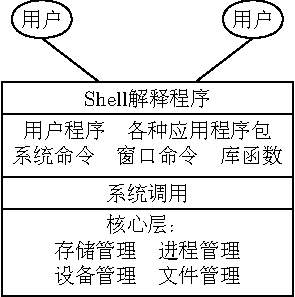
\includegraphics{graph/unix-0.pdf}
  \caption{Unix/Linux结构图(测试图形)}
  \label{fig:UnixTopo}
\end{figure}

\subsection{图片欣赏}
\label{subsec:picView}

下面给出几张美图看看。它们分别是Gnu的logo,内核Linux的logo,还有我最喜
欢的理查德的照片,最后一张是我在网上找到的,自己稍作了处理,嘻嘻……!

\begin{figure}[!htbp]
  \centering
  \subfloat[Gnu Logo]{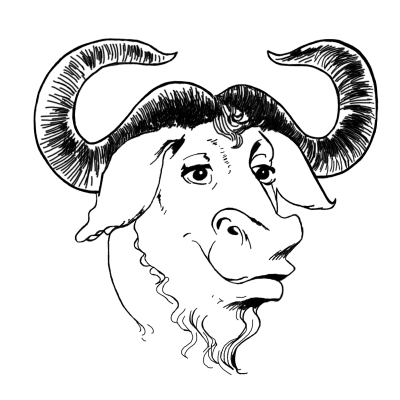
\includegraphics[width=.36\textwidth]{img/gnulogo.png}}
  \subfloat[Linux Logo]{
\includegraphics[width=.34\textwidth]{img/linuxlogo.png}}\hspace{30pt}
  \subfloat[Richard]{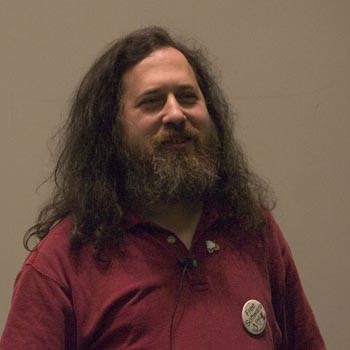
\includegraphics[width=.3328\textwidth]{img/stallman.jpg}}\vspace{10pt}
  \subfloat[网友恶搞]{
\includegraphics[width=.36\textwidth]{img/lw.png}}
  \caption{美图欣赏}
  \label{fig:meituxinshang}
\end{figure}

\section{本书使用的操作系统及环境}
\label{sec:thisOS}

本书的所有操作是在作者笔记本上的虚拟机上演示,虚拟机操作系统
为CentOS7u6 64位。

